% !TEX root = ..\main.tex
\chapter{State-of-the-Art}

This chapter presentes the state-of-the-art topics which is relevant to this research project. Section 2.1 looks into technical debt with its definitions, types etc. Section 2.2 looks into embedded systems and some of the challenges with it. Section 2.3 presents 


\section{Technical Debt}
The concept of technical debt was first introduced by Ward Cunningham in 1992 in order to communicate the problem with non-technical stakeholders\cite{p29-cunningham}. The concept was used to describe the system design trade-offs that are made everyday. In order to deliver business functionality as quickly as possible, 'quick and dirty' decisions leading to technical debt had to be made, which affects future development activities. Cunningham further describes technical debt as \textit{"shipping first time code is like going into debt. A little debt speeds development as long as it is paid back promptly with a rewrite"}. As time goes, technical debt accumulates interest leading to increased costs of a software system\cite{p31-guo,p35-klinger}. However, not all debts are necessarily bad. A small portion of debt might help developers speed up the development process in short term\cite{p31-guo}. 


%% The costs of technical debt
\begin{figure}
	\centering
	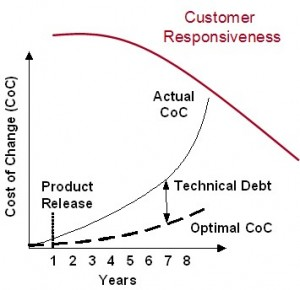
\includegraphics[width=0.8\textwidth]{images/techdebtCurve.jpg}
	\caption{The Technical Debt Curve\cite{jim-highsmith}}
	\label{fig:techDebtCurve}
\end{figure}

Figure \ref{fig:techDebtCurve} illustrates what happends as technical debt grows within a software product over time. Once we are on the far right of the curve, all choices are hard. The software controls us more than we control it.

%%%

\subsection{Comparation with financial debt}
Techincal debt has many similarities as financial debt\cite{p50-allman,Zazworka:2011:PDD:1985362.1985372}, which can be seen as the following:
\begin{itemize}
	\item You take a loan that has to be repaid later
	\item You usually repay the loan with interest
	\item If you can't pay back, a very high cost will follow. For example, you can loose your house or car.
\end{itemize}

Like financial debt, technical debt accrues interest over time which comes in the form of extra effort that have to be dedicated in future development because of bad choices\cite{p31-guo,p35-klinger}. You can choose to continue paying the interest, or you can pay down the debt by refactoring the code into something better which reduces interest payments in the future\cite{url-fowler}. If the debt is not repaid, development might slow down, e.g due to poor maintainability of the code. This can lead to software project failure and you might go bankrupt\cite{p50-allman}. 

There are some differences between financial and technical debt as well. The debt has to be repaid eventually, but not on any fixed schedule\cite{p50-allman}. This means that some debts may never have to be paid back, which depends on the interest and the cost of paying back the debt. The person who takes the debt is not necessarily the one who has to pay it off. A software project which moves from development mode to maintencance mode might change the engineers as well. So the engineers who has to maintain the system are the one who has to pay back the debt which occured in the development mode. Developers are often rewarded for their implementation speed. 
Technical debt is not only about bad code design. In practice, it's much more than that. Example on interests might be lower pace of development, low competitiveness, security flaws on the system, loss of developers and their expertise, poor internal collaboration environment, dissatisfied customers and loss of market share\cite{p50-allman}.

\subsection{Types of technical debt}
Since the original definition by Cunningham, numerous people have proposed definitions to the term technical debt. McConnels splits the term into two categories based on how they are incurred, intentionally or unintentionally\cite{url-mcconnell}. The unintentional category includes debt that comes from doing a poor job. For instance, uninntentional debt might be when a junior software developer writes bad code due to lack of knowledge and experience. Intentional debt occurs when an organization makes a decision to optimize for the present rather than the future. An example is when the project release must be done on time, or else there wont be a next release. This leads to bad decisions, like taking a shortcut to solve a problem, and reconcile the problem after shipment

Fowlers presents a more formal explanation of how techincal debt can occur\cite{url-fowler}. He categories technical debt into different debt types, in which he calls \textit{"Technical Debt Quadrant"}. As seen in the Figure \ref{fig:techDebtQuad}, the debt is grouped into four categories: 

\begin{itemize}
	\item \textbf{Reckless/Deliberate debt}: The team feels time pressure, and takes shortcuts intentionally without any thoughts on how to address the consequences in the future.
	\item \textbf{Reckless/Inadvertent debt}: Best practices when it comes to code and design is ignored, and a big mess in the codebase is made.
	\item \textbf{Prudent/Deliberate debt}: : The value of taking shortcuts is worth the cost of incurring debt in order to meet a deadline. The team is aware of the consequences, and has a plan in place to address them in the future. 
	\item \textbf{Prudent/Inadvertent debt}: Software development process is as much learning as it is coding. The team can deliver a valuable software with clean code, but in the end they might realize that the design could have been better.
\end{itemize}

\begin{figure}
	\centering
	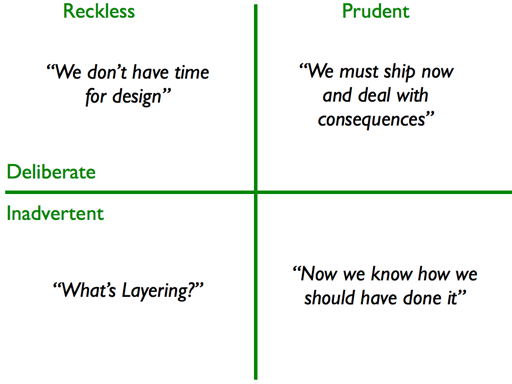
\includegraphics[width=0.8\textwidth]{images/techDebtQuadrant.png}
	\caption{Technical Debt Quadrant}
	\label{fig:techDebtQuad}
\end{figure}

Krutchen divides technical debt into two categories\cite{krutchen}. Visible, debt that is visible for everyone. It containts elements such as new functionality to add and defects to fix. Invisible is the other category, debt that is only visible to software developers.


\subsection{Causes}
Many thinks that technical debt is mostly related to code decide. However, technical debt might occur already in the requirement specification phase in software development project. 

While financial debt occus from deliberate actions of taking a loan, technical debt may be caused by several factors. Antares categories these factors into four groups:
\begin{itemize}
	\item Work processes: Software development methology, can some tasks be automized (with a deploy script), is tests written after bug fixing, do you map and document shortcuts you take, is there any plans for techincal debt management later, is it important to implement new functionality or to make sure that the existing ones work propertly?
	\item People (knowledge and capacity): Do you need some individuals to finish a task, Do you have the right people for the job, is enough training given to new people, what happens if you need someone who's on vacation/change project/is sick or something. You should keep this in mind and make a plan on how knowledge is transferred. Techcnical debt can be the reason for poor motivation and productivity which causes you to work poorly. 
	\item Technology: Is solutions hard to integrate with other solutions, is all the systems out there compatible with newer technology, is there any outdated or duplicated code in the system, is all the systems secure, is the solutions old, or user friendly, is there some code which is hard to maintencance. 
	\item Collaboration in the organization: Commuinication between developers and requirement people. You often get a list with requirements, is the list understandable? Do we work with a backlog with tasks that should have been solved long time ago, but not which is not "actual" now?
\end{itemize}
Developers might not care about the product because they don't feel that they "own" what's being made. They get told what do to, but not more than that. Can't make requirements.


Operating technical debt might be to maintenance and manage existing code rather than implementing new functionality. It is important to keep track of the technical debt, and incur interest payments, before it makes troubles for you. Do do that, you could for example set up a plan for repayment which tells you something about how the debt shall be repayed. Scrum can be used to do this for example, where you split the repayment plan to smaller parts where you estimate and prioritize tasks. It is important to remember that taking too much loan might cause problems. As mentioned ealier, technical debt can be seen as taking a financial loan according to Cunningham. The loan has to be repaid with interests. Technical debt uses time and effort as repayment. It is acceptable to take a loan, but it should be controlled. Do not take loan than what you are able to handle. Think with your head.

Main developers behind a software project aren't the one who usually maintain the code. Companies often has policies where they transfer a project to new developers after the development phase is over. The reasons could be to save money, or that the new developers might work more. These maintenance people often haas to repay the debt. The main developers gets awarded for their implementation speed rather than thinking on maintanence and evolution. They can often be placed on new projects before the debt has to be paid back, making them unavaiable for a period. Too few systems also has TODO or FIXME comments in their source code.

%Når det kommer til teknisk gjeld er det ikke alltid personen som har utviklet noe som tar ansvar, men kan en annen kan ta seg av den gjelda. Mange utviklere vedlikeholder ikke sin egen kode. Mange selskaper har også regler om at når et software er ferdig utviklet av de "beste" til å bli vedlikeholdt av de nest beste, som ofte kan få mindre betalt men har mye mer arbeid å gjøre. Ingen i din organisasjonen viser interesse for det, er brukerne som må betale for gjelda. Utviklere er belønnet for hvor raskt de implementerer enn langsiktig vedlikehold og kan ha fått seg et nytt prosjekt før gjelda er betalt. Få systemer har TODO eller FIXME kommentarer i kildekoden. 

\subsection{Measuring technical debt}
Define technical debt in your backlog.
Use tools like Sonar, SQALE.

Technical debt isn't the problem, but it can be seen as a symptom of a potential problem. THings might go wrong with the organization which is causing techncial debt. Business processes, operational, business methods. 


\subsection{Technical debt in Industry}
Technical debt today is connected with many differnet aspects in the software development process, like documentation debt, requirements debt, architecture debt etc\cite{Falessi:2015:FRI:2797433.2797462}. 

All development results in some amount of technical debt. The challenge is to manage it, reduce it and develop practices to keep it at a level that does not impact performance and availability of your critical business services.

Using sequential design processes in software development processes to build complex, intensive systems is often a failure. Requirements are specified at the beginning of the software development process, and the remaining software development activities has to follow the initiral requirements. This kind of model is not appropiate to use for big softwares where technology and business requirements always change. This is why agile methods was made, where change and feedback is important. One of the benefits is the ability to quickly release new functionality. However, one of the problems with agile methods is that developers often wants to focus on implementing new fucntionality, which results in poor focus on design, code quality, testing, which again leads to technical debt.  

Klinger carried out an industrial case study at IBM where four technical architechts with different backgrounds were interviewed and the goal was to examine how the decisions to incur debt was taken and the extend to which the debt provided leverage\cite{p35-klinger}. What they found out was that the company failed to assess the impact of intentionally incurring debt on projects. Decisions regarding technical debt were rarely quantified. There were also big organizational gaps among the business, operational and technical stakeholders, which incurred debt.

Codabux carried out an industrial case study where the topic was agile development focusing on techincal debt\cite{p8-codabux}. They wanted to gain insights on agile adoption and how techincal debt affects the development processes. This industiral case study happened in form of an interview. After conducting the research, they got two definitions of technical debt, further known as infrastructure and automation debt. Infrastrucutre is the work that improves the teams processes and ability to produce a quality procudt with refactoring, repackaging, developing unit tests. Automation isthe work relatedd to supporting continious integration and faster development cycles. The term technical debt was mostly related to design, testing and defect debts according to the participants. One of the engineers mentioned that when they were working, they didn't know the "balacne of the credit card. They kept charging it". Management decides when enough debt has incurred, and is influenced by the customer needs.



\subsection{Organizational debt}
While technical debt is known problem, there's one more type of debt which can be accrued on a compandy-wide level. This type of debt is called organizational debt. Organizational debt is all about people and culture compromises made to \textit{'just get it done'} in early stages of a startup, preventing a company from running smoothly\cite{steve-blank}. When things should be going great, organizational debt can turn a growing company to a nightmare. Growing companies needs to know how to recognize and refactor organizational debt. 

Some of the causes behind organizational debt might be:

\begin{itemize}
	\item Training the new hires, both culture and specific tasks
	\item Retain existing hire by doing something for them. Many doesn't get promoted. New hire might get a better posistion than existing hire who has been there from the start.
\end{itemize}

Sometimes, the employees gets awarded by good building, new furnitures, and compensation for executive staff. However, that isn't enough. Think about existing employees who's been there from the start. You might end up loosing qualified people who's spent years building up the company, but not compensated for it. Top-down approach is focused too much. Think about the bottom employees.They have the inistituinal knowledge and hard-earned skills.

When new people got hired, the ones who could train them about the company culture and how to do their specific tasks is the old employees who's being underpaid. They will look for another job. No one would be able to train the new people then. Giving compensation in form of stock vesting, insurance benefits, movie nights etc isnt enough as everyone gets it. Do something for the employees who's been there for a long time.

Refarocting might be important in order to reduce the organizational debt. Write plan for managing new wave of hires before hiring them. Sometimes, you'll also need to think about what you will have to do if you're about to loose a key employee. Is it worth to replace employees who hold critical knowledge? Put together an expence budget using the current employee salaries. See who's important. Identify the one they wanted to keep and upgrade them. Some employees might not be that important as welll as they might be a performance problem for the whole organization. Need to look at the company culture as well, does it take into account of the new size and stage of the organization? What have the company achieved, what are the key elements that have made it great so farm, are they same of different. Think about the customer too. Does we talk to the customer, or does the customer talk to us. Also, keep in mind that an adivosory board of other CEOS who've been through the early stages might be good. Failure to refactor might kill a growing company\cite{steve-blank}.

Some examples on organizational debt:
\begin{itemize}
	\item Different departments solving the same problems might use differnet methologies and tools. Difficult to see similarities in order to address company-wide issues.
	\item Creation of processes and implement solutions which seems great at first, but didnt address the root casue of the issue and ending up creating more problems.
	\item Time constraints, solving a problem in less-than-ideal manner this time. This manner is repeated because no one remember that the first time was intended to be one-off situation.
\end{itemize}



%%%%%%%%%%%%%%%%%%%%%%%%%%%%%%%%%%%%%%%%%%%%%%%%%%%%%%%%%%%%%%%%%%%%%%%%%%%%%%%%%%%%%%




\section{Embedded Systems}
%https://www.quora.com/What-are-the-characteristics-of-embedded-system

\textit{IEEE Standard Glossary of Software Engineering Terminology}\cite{159342} defines an embedded system as:
\begin{displayquote}
	\textit{A computer system that is part of a larger system and performs some of the requirements of that system; for example, a compyter system used in an aircraft or rapid transit system.}
\end{displayquote}

While traditional computers are designed for performing multiple tasks, embedded systems are designed to perform a specific task under certain constraints. Due to the certain contraints, embedded systems are known as safety-critical systems and hard-real-time systems [9][10]. 




It is fairly safe to assume that a bsuiness in the coming years will be much more connected to the outside worl than it is now. This connectivity might come through mobile applications, social networks or the clouds. 

If legacy software can be maintaned to an acceptable level


\subsection{Embedded system software}

Embedded software is a computer software for embedded systems. It is specialized for a type of hardware which it lays and runs on. Therefore, embedded software might have multiple constraints related to run-time, memory usage, processing power etc.

Embedded systems is part of a large share of today's products. While developing embedded system software, quality is a key characteristic. Managing software quality is necessary to deliver software in a useful, safe and reliable way [7]. 

 
Embedded software had an important role today with the rapid evolution of ES. Escpecially with the Internet of Things trend.

However, there are some challenges with embedde system software. These type of software usually has long lifetime. Old systems are usually hard to maintain compared to new ones. Companies must maintain many different configurations, and maintaining systems are challenging due to time. It is important to take the right choices when designing such systems. Abstract and high level design, architecture. People tend to deliver something in time rather than making something good. 

\subsection{Security}


\subsection{Virtualization of embedded systems}


%%%%%%%%%%%%%%%%%%%%%%%%%%%%%%%%%%%%%%%%%%%%%%%%%%%%%%%%%%%%%%%%%%%%%%%%%%%%%%%%%%%%%%


\section{Configuration management}

Dart defines configuration management as a dicipline for controlling the evolution of software systems (siter dart). This includes content, changes and status in a shared project. Both processes and technical solutions to handle changes and the projects integrity. Example, if a new version of the product is released, everything related to this projects needs to be up-to-date. Like documentation. Configuration management identifies every component in a project and has an overview of every suggestions and changes from day 1 to the end of the product. Some examples on SCM is Git-SCM, SVN, RCS, Adele, ClearCase. Version control is the key behind SCM. IEEE standard 729-1983 highlights the following operational aspects of CM:

\begin{itemize}
	\item \textbf{Idenfitication}: The products structure. Identifies every component in the products, making them unique and accessible in some form.
	\item \textbf{Control}: Controls every reelase and changes of a product throghout the lifecycles by having some controls in place that ensure consistent software via the creation of ab aseline product.
	\item \textbf{Status accounting}: Records and reports the status of components and change requests. It is also possible to review statistics about components in the product.
	\item \textbf{Audit and review}: Validates the product and maintaining the consistency between components by ensuring that the product is a well-defined collection of compontens.
\end{itemize}

In addition to those aspects, we can extend the definition of CM by three more aspects
\begin{itemize}
	\item \textbf{Manufacture}: Maintaining the construction, and build the product in an optimal way.
	\item \textbf{Process management}: Take care of the companies policies, processes and lifecycle model.
	\item \textbf{Teamwork}: Review the work and make sure that the collaboration is good. Keep an eye on the interaction between multiple users and the product.

\end{itemize}

Choosing a robust SCM system makes it possible to deal with big and complex files. It also supports distributed development. The right combination of SCM system and best practices makes it possible for embedded development projects to progress fast and efficiently. 

Some of the challanges related to development of embedded systems:
\begin{itemize}
	\item \textbf{Complex file sets}: Embedded systems consists of multiple diverse components, both hardware and software. This makes the system complex. Embedded system may also have different adjustable compoents for a specific platform, makin it easier to sell a product by tweaking some parameters. Dealing with these variates is a major challenge. Another challenge is that a product requires correct version of a component. Ensuring the consistency between components and their dependens files is a challenge as well.
	\item \textbf{Distributed teams}: Components may be developed in different places in our worl. Two team might for example work on the same components, especially when development are being outsourced. Such collaboration needs every developer to access each others work. The challenge is keep the team syncronized. 
	\item \textbf{Management and versioning of intellectual property}: Embedded systems, or software generally might use third-party technologies. It is important that those technologies are up-to-date, and maintained. These updates needs to be tracable such that each components has the right, compatible and stable version of its software. If something is not outsourced, it might be a challenge for developers to contribute and trace their changes.
\end{itemize}



\section{DevOps}
Continious Integration, Continious Delivery, Automation, Deployment



%%%%%%%%%%%%%%%%%%%%%%%%%%%%%%%%%%%%%%%%%%%%%%%%%%%%%%%%%%%%%%%%%%%%%%%%%%%%%%%%%%%%%%

\section{Software Architecture}
Bass, Klements and Kazman\cite{Bass:2012:SAP:2392670} defines software architecture as following: 

\begin{displayquote}
The software architecture of a system is teh set of structures needed to reason about the system, which compromise software elements, relations among them, and properties of both.
\end{displayquote}

The architecture of a software is one of the most important artifacts within the systems life cycle\cite{Bass:2012:SAP:2392670,knodel2006static}. Architectural design decisions that are made during the design phase affects the systems ability to accept changes and to adapt to changing market requirements in the future. As the design decisions are made early, it will directly affect the evolution and maintenance phase\cite{Pressman:2009:SEP:1593949}, activities that consumes a big part of the systems lifespan\cite{Vliet:2008:SEP:1481475}. 
%As the system evolves over time, it will go through lots of changes. This could be like bugfixes, implementation of new features, 

Architectural drift - the architectural documentation is updated according to implementation, but ends up as an architecture without vision and direction.
Architectural erosion - the implementation drifts away from the planned architecture so they are no longer consistent. 




\section{Software development methods} % (fold)

\begin{figure}
	\centering
	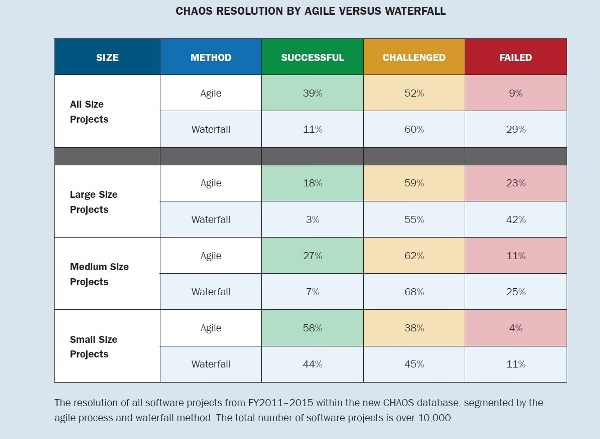
\includegraphics[width=0.8\textwidth]{images/Agile-Waterfall-Success-Failure-Rates.jpg}
	\caption{The CHAOS Manifesto, The Standish Group 2012}
	\label{fig:agileWaterfallSuccessFailureRates}
\end{figure}



\subsection{Waterfall}

\subsection{Agile}


\subsection{V model}

\subsection{Prototyping}

\subsection{Test-driven development}


\section{Software maintenance and evolution}
Increasingly, more and more software developers are employed to maintain and evolve existing systems instead of developing new systems from scratch "trenger sitat". Software evolution is a process that usually takes place when the initial development of a software project is done and was successful\cite{Bennett:2000:SME:336512.336534}. The goal of software evolution is to incorporate new user requirements in the application and adapt it to the existing application. This phase is important beacuse it takes a lage part of the overall lifecycle costs. It is also important because these days technology tend to change rapidly, and not following these trend means loosing business oppertunities.

IEE 1219 defines software maintenance as follows\cite{720567}:
\begin{displayquote}
Modification of a software after delivery to correct faults, to improve performance or other attributes, or to adapt the product to a modified environment.
\end{displayquote} 
Maintenance can be classified into four types\cite{Bennett:2000:SME:336512.336534,720567}.

\begin{itemize}
	\item Adaptive: Modification of a software product performed after delivery to keep a computer program usable in a changed or changing environment.
	\item Perfective: Modification of a software product after delivery to improve performance or maintainability.
	\item Corrective: Reactive modification of a software product performed after delivery to correct discovered faults.
	\item Preventive: Maintenance performed for the purpose of preventing problems before they occur.
\end{itemize}

According to van Vliet, the real maintenance activity corrective maintenance\cite{Vliet:2008:SEP:1481475}. 50\% of the total software maintenance is spent on perfective, 25\% on adaptive maintenance, and 4\% on preventive maintenance. This leads to that 21\% of the total maintenance activity is corrective maintenance, the 'real' maintenance\cite{Vliet:2008:SEP:1481475}. This hasn't changed since the 1980s when Lientz and and Swanson conducted a study on software maintenance\cite{lientz1980software}. Their study found out that most severe maintenance problems was caused by poor documentation, demand from users for changes, difficulty meeting schedulment, and problems training new hires.  Some other problem areas was lack of user understand and user training, the customers didnt understand how system works. Programmers had low productivity, skill level and motivation. System was badly designed leading to low quality. 

As a system changes over time, it will have impact on the systems internal structure and complexity. Software evolution might cause poor software quality and erosion of software architecture over time\cite{Bass:2012:SAP:2392670}.


\begin{figure}
	\centering
	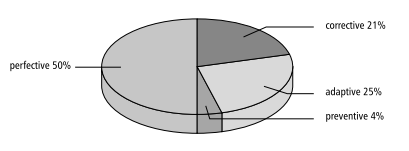
\includegraphics[width=0.8\textwidth]{images/maintenance.png}
	\caption{Distribution of maintenance activities\cite{Vliet:2008:SEP:1481475}}
	\label{fig:maintenanceActivities}
\end{figure}

\section{Software reuse}
Software reuse is the process of using existing software artifacts, or knowledge, to create new software, rather than building it from scratch. Software reuse is a key method for improving software quality\cite{frakes1996software}. 

\section{Refactoring}
Design debt, a specific type of technical debt, accumulates as you write code\cite{Zazworka:2011:PDD:1985362.1985372}. This type of debt can be reduced when you refactor. Fowler defines refactoring as means of adjusting the design and architecture towards new requirements without changing the externial behaviour of a program in order to improve the quality of the system\cite{1999:RID:311424}. It is an act of improving the design of an existing system\cite{Vliet:2008:SEP:1481475}. Most of the time in spent on reducing design debt is on refactoring activities itself. These activities includes planning the design and architecture, rewriting the code, and adjusting documentation\cite{Pressman:2009:SEP:1593949}. It is believed that refactoring is one of the key methods to reduce technical debt in a system ("siter").  





